
\documentclass[11pt, titlepage, oneside, a4paper]{article}
\usepackage[T1]{fontenc}
\usepackage[utf8]{inputenc}
\usepackage[english]{babel}
\usepackage{amssymb, graphicx, fancyhdr}
\addtolength{\textheight}{20mm}
\addtolength{\voffset}{-5mm}
\renewcommand{\sectionmark}[1]{\markleft{#1}}

% \Section ger mindre spillutrymme, använd dem om du vill
\newcommand{\Section}[1]{\section{#1}\vspace{-8pt}}
\newcommand{\Subsection}[1]{\vspace{-4pt}\subsection{#1}\vspace{-8pt}}
\newcommand{\Subsubsection}[1]{\vspace{-4pt}\subsubsection{#1}\vspace{-8pt}}
	
% appendices, \appitem och \appsubitem är för bilagor
\newcounter{appendixpage}

\newenvironment{appendices}{
	\setcounter{appendixpage}{\arabic{page}}
	\stepcounter{appendixpage}
}

\newcommand{\appitem}[2]{
	\stepcounter{section}
	\addtocontents{toc}{\protect\contentsline{section}{\numberline{\Alph{section}}#1}{\arabic{appendixpage}}}
	\addtocounter{appendixpage}{#2}
}

\newcommand{\appsubitem}[2]{
	\stepcounter{subsection}
	\addtocontents{toc}{\protect\contentsline{subsection}{\numberline{\Alph{section}.\arabic{subsection}}#1}{\arabic{appendixpage}}}
	\addtocounter{appendixpage}{#2}
}

% Ändra de rader som behöver ändras
\def\inst{Datavetenskap}
\def\typeofdoc{Laborationsrapport}
\def\course{Systemnära Programmering 7,5 hp}
\def\pretitle{Laboration 4}
\def\title{mish}
\def\name{Christer Jakobsson}
\def\username{dv12cjn}
\def\email{\username{}@cs.umu.se}
\def\path{edu/sysprog/lab4}
\def\graders{Mikael Rännar, Adam Dahlgren Lindström, Niklas Fries, Oskar Ottander}


% Om du vill referera till katalogen där dina filer ligger kan du 
% använda \fullpath som kommer att vara "~username/edu..." o.s.v.
\def\fullpath{\raisebox{1pt}{$\scriptstyle \sim$}\username/\path}


% Här brjar själva dokumentet
\begin{document}

	% Skapar framsidan (om den inte duger: gör helt enkelt en egen)
	\begin{titlepage}
		\thispagestyle{empty}
		\begin{large}
			\begin{tabular}{@{}p{\textwidth}@{}}
				\textbf{UMEÅ UNIVERSITET \hfill \today} \\
				\textbf{Institutionen för \inst} \\
				\textbf{\typeofdoc} \\
			\end{tabular}
		\end{large}
		\vspace{10mm}
		\begin{center}
			\LARGE{\pretitle} \\
			\huge{\textbf{\course}}\\
			\vspace{10mm}
			\LARGE{\title} \\
			\vspace{15mm}
			\begin{large}
				\begin{tabular}{ll}
					\textbf{Namn} & \name \\
					\textbf{E-mail} & \texttt{\email} \\
					\textbf{Sökväg} & \texttt{\fullpath} \\
				\end{tabular}
			\end{large}
			\vfill
			\large{\textbf{Handledare}}\\
			\mbox{\large{\graders}}
		\end{center}
	\end{titlepage}


	% Fixar sidfot
	\lfoot{\footnotesize{\name, \email}}
	\rfoot{\footnotesize{\today}}
	\lhead{\sc\footnotesize\title}
	\rhead{\nouppercase{\sc\footnotesize\leftmark}}
	\pagestyle{fancy}
	\renewcommand{\headrulewidth}{0.2pt}
	\renewcommand{\footrulewidth}{0.2pt}

	% Skapar innehållsförteckning.
	% Tänk på att köra latex 2ggr för att uppdatera allt
	\pagenumbering{roman}
	\tableofcontents
	
	% och lägger in en sidbrytning
	\newpage

	\pagenumbering{arabic}

	% I Sverige har vi normalt inget indrag vid nytt stycke
	\setlength{\parindent}{0pt}
	% men däremot lite mellanrum
	\setlength{\parskip}{10pt}

	% Lägger in rubrik (finns \section, men då får man mycket spillutrymme)
	\Section{Problemspecifikation}
		% \emph innebär emphasize, d.v.s. betona eller framhåll -> kursiv stil
		\emph{Denna laborations syfte har varit att få praktisk erfarenhet av att använda fork och andra systemanrop i linux, samt att använda fil deskriptorer för att omdirigera standard in och standard out}

		% lägg in en underrubrik (\subsection -> spillutrymme)
		\Subsection{Problemsammanfattning}
		Denna laboration har gått ut på att skapa ett minimalt \emph{shell} (kommandoskal). Ett skal är ett program som körs
		då man öppnar en terminal, det skriver ut en prompt och väntar på kommandon att exekvera. 
		
		De funktioner som skalet skall klara av är:
		\begin{itemize}
		 \item Exekvering av kommandon och program
		 \item Pipor mellan program
		 \item Omdirigering av standard input och standard output
		 \item Hantera signalen SIGINT. Vid signal, avbryta exekveringen av alla uppstartade program.
		\end{itemize}

		\Subsection{Originalspecifikation}
			Specifikationen i sin helhet finns på\\
                        \verb!http://www8.cs.umu.se/kurser/5DV088/HT14/lab/lab4/!

	\Section{Åtkomst och användarhandledning}
		
		\Subsection{Filer som ingår i lösningen}
			I katalogen \texttt{\fullpath} ...
		
		\begin{itemize} 
		 \item[mish.c] Fil som är huvuddelen i programmet.
		 \item[mish.h] Header fil för \emph{mish.c}
		 \item[execute.c] Innehåller två funktioner som ingick i uppgiften att implementera.
		 \item[execute.h] Header fil till \emph{execute.c}
		 \item[parser.c] Given fil för uppgiften, behandlar en kommandorad och skapar structar med information om varje kommando.
		 \item[parser.h] Header fil till \emph{parser.c}
		 \item[sighant.c] Signal hanterare till \emph{mish}
		 \item[sighant.h] Header fil till \emph{sighant.c}
		 \item[makefile] make fil för att kompilera alla delar till programmet och skapa ett körbart \emph{mish}
		\end{itemize}

		\Subsection{Kompilering och körning}
		För att kompilera så använder man medföljande makefil och kör den genom att stå i samma mapp som filerna finns i och skriva
		\emph{make}. Detta kommer att kompilera de filer som inte har kompilerats förut och skapa ett exekverbart program som heter \emph{mish}.
		
		För att exekvera programmet skriver man i terminalen \emph{./mish}. Detta kommer att starta programmet och det kommer att skriva ut en prompt
		med aktuell katalog som programmet befinner sig i följt av \emph{:mish}. Nu så väntar mish på att användaren ska skriva in ett kommando och när användaren trycker Enter
		så försöker mish att köra kommandot, visar ett felmeddelande om något fel uppstår. 
		
		Programmet avslutas när det får signalen \emph{EOF} (End-Of-File), vilket kan göras genom att trycka CTRL + D.

	\Section{Systembeskrivning}
		\emph{I detta avsnitt beskrivs systemet i sin helhet mer i detalj.
			Datastrukturer och annan intern representation som är central
			för uppgiftens lösning behandlas. Dessutom beskrivs de olika
			komponenternas relationer till varandra.}
		
		
		%Dessa rubriker behöver inte finnas med, men något i denna stil
		%bör det kanske vara
		\Subsection{Systemöversikt}
		\subsubsection{mish}
		\emph{mish} är huvuddelen i programmet, börjar med att skriva ut en prompt som en vanlig terminal och väntar på kommandon, Detta är i en while loop
		som kommmer att iterera ända tills användaren ger programmet EOF varpå programmet avslutas. Användaren kan här skriva ett kommando och när 
		Enter trycks så skickas den rad som användaren skrivit in till den givna parsern som tolkar raden och bygger upp en array innehållande structs för varje kommando.
		Programmet försöker sedan att exekvera de kommandon den har fått,
		om någon av kommandona inte var ett riktigt kommando eller om kommandot får felaktiga parametrar så kommer det inte kunna exekveras och ett felmeddelande
		skrivs ut och prompten skrivt ut igen. Om det var en giltig kommandorad så kommer parsern att dela upp varje kommando och skapa en struct för varje 
		kommando som ska exekveras och skapa en array av dessa structar. Structen innehåller information om kommandot, om det har en in eller utfil samt vilka parametrar som
		kommandot ska exekveras med. 
		
		Med denna array av structar så itererar jag igenom alla kommandon och kollar om kommandot som skall köras antingen är \emph{echo} eller \emph{cd}.
		Om så är fallet så sätts den aktuella structens variabel \emph{internal} till ett värde som sedan kontrolleras innan kommando exekvering och kör det
		interna kommandot om det matchade. 
		Sedan så loopas arrayen av kommandon igenom och för varje kommando så skapas en kopia av processen som körs och dess standard input och/eller standard 
		output  omdirigeras för att skapa pipor emellan alla kommandon som ska exekveras. Kontrollerar även om standard in/out ska omdirigeras ifrån eller till
		en fil för kommandot.
		
		
		
		\subsubsection{sighant}
		Denna fil är en signal hanterare vars uppgift är att döda alla barnprocesser till \emph{mish}  om användaren skickar SIGINT. 
		Detta görs genom att \emph{mish} skickar SIGINT till barnen och för att försöka avbryta dem. Innehåller två globala variabler som håller reda på varje barns process id, en array som lagrar alla pids 
		och en int som är antalet barnprocesser. Dessa globala variabler används sedan i mish filen som stoppar in pids i arrayen och ändrar heltalet som innehåller hur många barnprocesser så det är korrekt antal.
		\subsubsection{execute}
		Denna fil implementerar de två funktioner vars huvuden angivits i \emph{execute.h}. En funktion som duplicerar en pipa till standard in/out och en som 
		omdirigerar standard in/out till eller ifrån en fil.
		\subsubsection{Givna filer}
		\emph{För att förenkla laborationen så är en del filer givna som ska hjälpa mig att bygga skalet.} 
		
		\begin{itemize}
		 \item[parser] Denna fil tar kommandoraden som användaren skrivit in, behandlar den och bygger upp en array av Command structar.
		 Varje struct i arrayen innehåller information om vilket kommando som ska köras, med vilka argument och om det datat ska hämtas eller 
		 skrivas från en fil.
		 \item[execute.h] Denna fil är till för att jag ska implementera två funktioner. En funktion som ska duplicera en pipa till en standard I/O fil deskriptor samt en funktion som
		 ska omdirigera läsning/skrivning från eller till en fil.
		\end{itemize}
		\newpage
		
		\Subsection{Anropningsdiagram}
		\emph{Figure \ref{fig:anropa} visar ett diagram över hur funktioner i programmet anropar varandra och vad de returnerar.}
		
		\begin{figure}[h]
		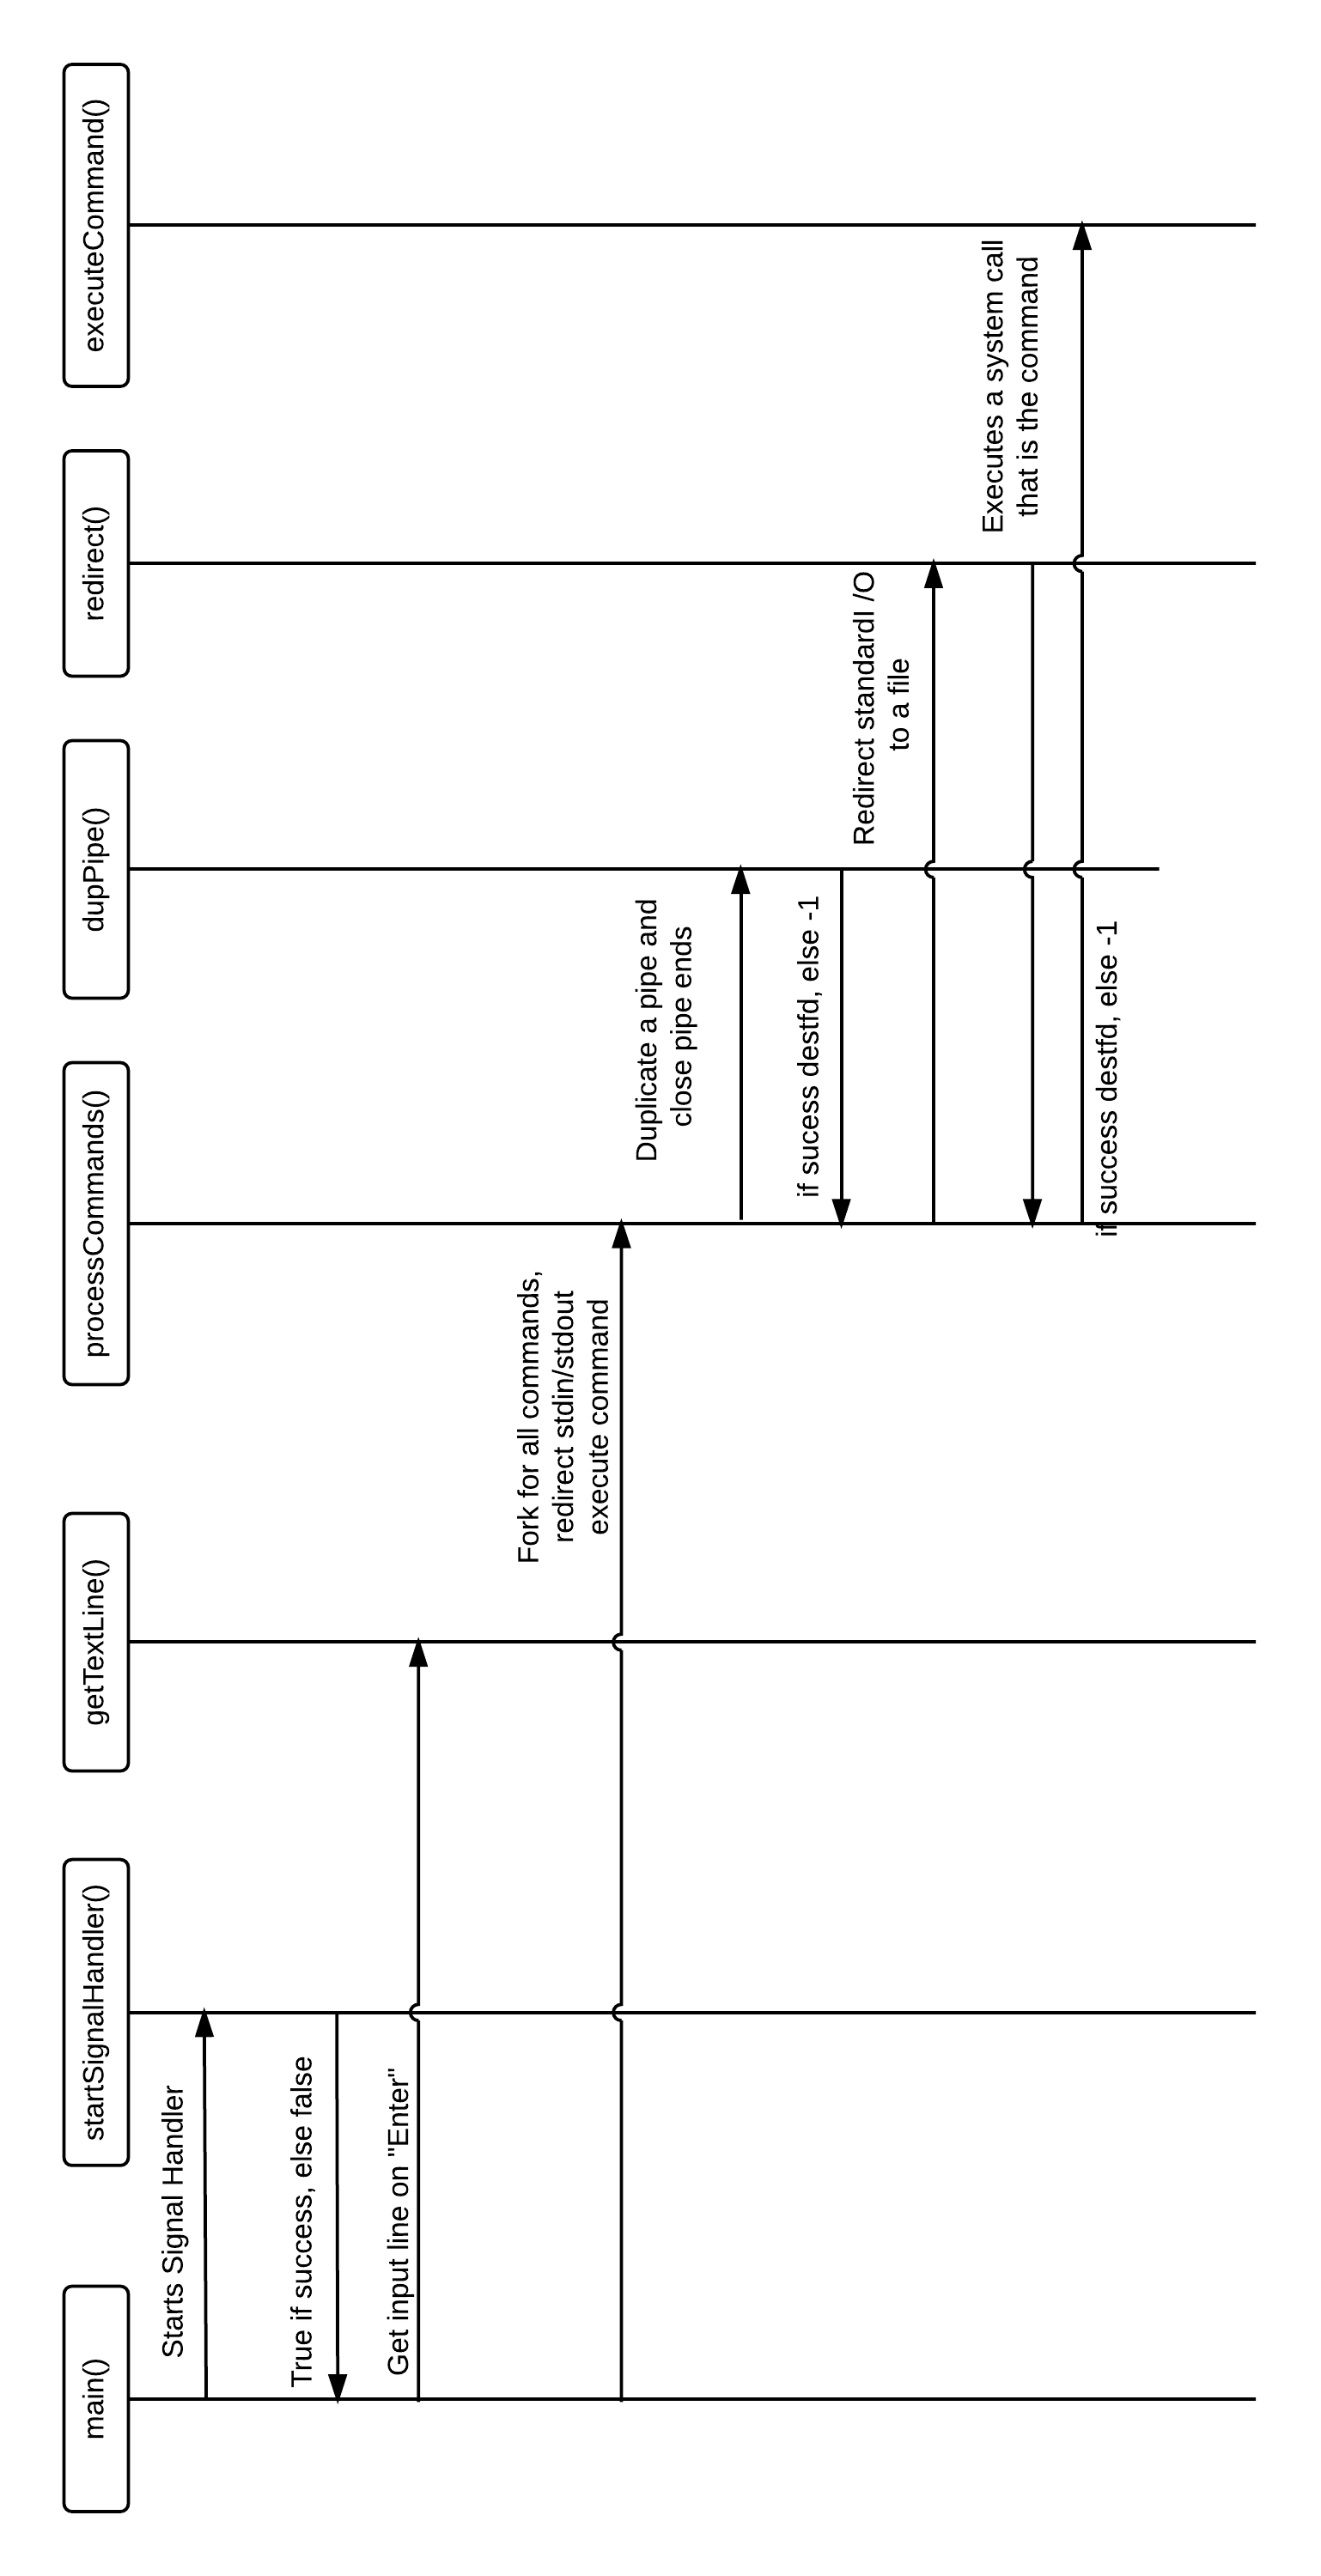
\includegraphics[width=0.6\textwidth]{anrop.png}
		\caption{Anropsdiagram}
		\label{fig:anropa}
		 \end{figure}
		
		\newpage
		
		\Subsection{Processkommunikation}
		För varje process som ska köras så görs en fork, detta skapar en barnprocess till \emph{mish} och barnet kommer då att
		omdirigera sin standard in/out beroende på hur kommandot som användaren skrev in såg ut och därefter kommer barnet att exekvera
		det systemanrop som det fått av struct arrayen.
		
		
		\emph{En omdirigering av standard in, så programmet läser från infil}
		\\Kommando: \textbf{wc < infil}
		\begin{figure}[h]
		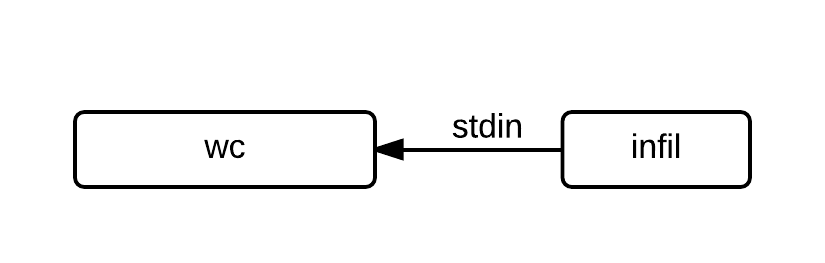
\includegraphics[width=0.8\textwidth]{infil.png}
		\caption{wc < infil}
		 \end{figure}	
		
		\emph{En omdirigering av standard out, så ls skriver till utfil}
		\\Kommando: \textbf{ls > utfil}
		\begin{figure}[h]
		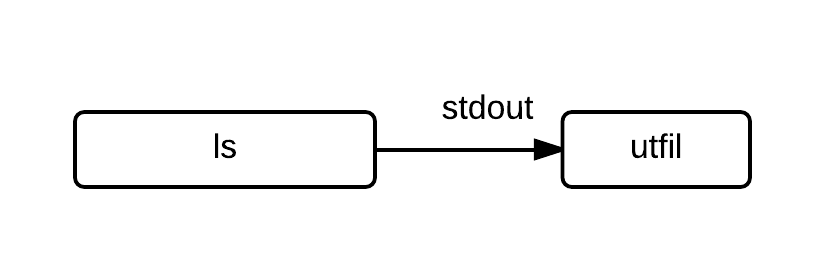
\includegraphics[width=0.8\textwidth]{utfil.png}
		\caption{ls > utfil}
		 \end{figure}
		 
		 \emph{En pipa mellan ls och wc, gör så att ls utdata kommer att läsas av wc.}
		 \\Kommando: \textbf{ls | wc}
		 \begin{figure}[h]
		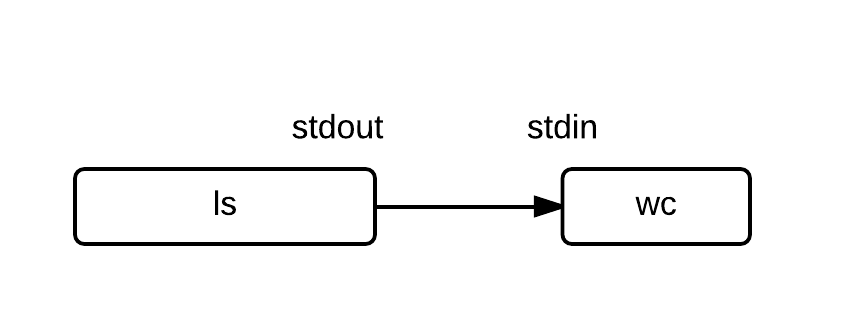
\includegraphics[width=0.8\textwidth]{pipa.png}
		\caption{ls | wc}
		 \end{figure}
		 
		  \emph{Ett kommando som använder sig av en pipa, en infil och en utfil}
		 \\Kommando: \textbf{ls | wc}
		 \begin{figure}[h]
		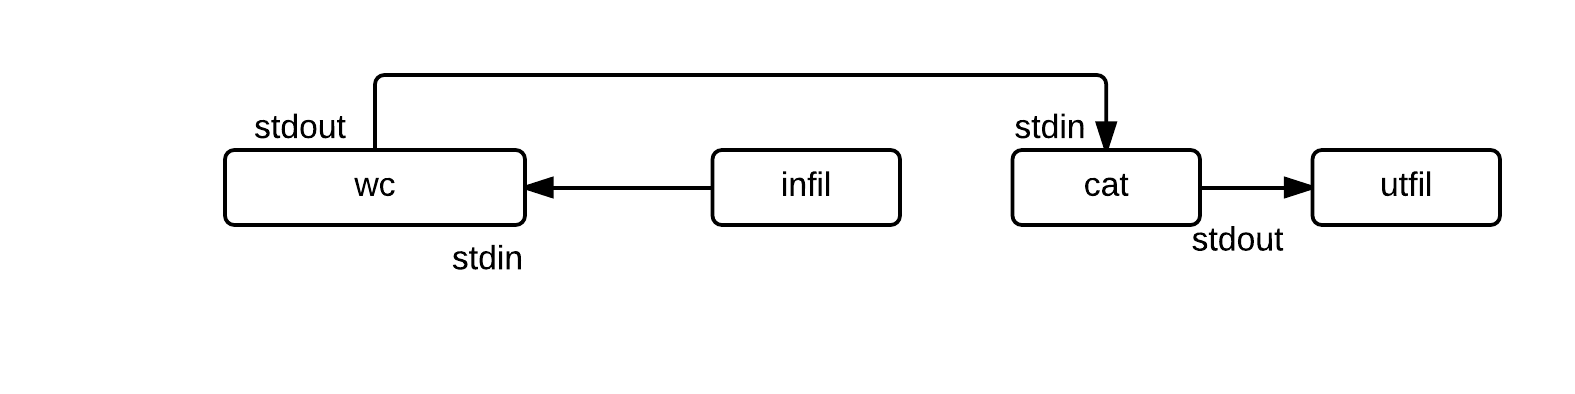
\includegraphics[width=0.8\textwidth]{allThings.png}
		\caption{wc < infil | cat > utfil}
		 \end{figure}

	\Section{Lösningens begränsningar}
		\emph{I detta avsnitt beskrivs alla begränsningar som lösningen av
			uppgiften innehåller. Detta innefattar även funna begränsningar
			som strider mot specifikationen.}
		
		Om användaren skriver \emph{fil > fil2} dvs att \emph{fil} ska skriva till \emph{fil2} vilket ej kan fungera för att \emph{fil} är en fil inte ett kommando som gör något så kommer 
		fil2 ändå att skapas.
		
		En begränsning är att \emph{mish} inte stödjer piltangenter såsom en vanlig terminal gör att man kan flytta positionen man skriver på och ta bort tecken mitt i det man skrivit.
	      
	      
		Ännu en begränsning är att \emph{mish} inte stödjer historik funktionen som de vanliga terminalerna använder sig av att man med hjälp av upp och ner piltangenterna kan blädda
		igenom vad man skrivit förr.
\end{document}